\section{Procedure Interface}

Procedure calls in XMP are the same as the base language. Procedure
calls between different languages and external library are also possible
if the base language supports them. 

In the below example, sub1() calls sub2() with a distributed array as an
argument.

\begin{XCexample}
void sub1(){
#pragma xmp nodes p[2]
#pragma xmp template t[10]
#pragma xmp distribute t[block] onto p
  double x[10];
#pragma xmp align x[i] with t[i]
  sub2(x);
}

void sub2(double a[10]){
#pragma xmp nodes p[2]
#pragma xmp template t[10]
#pragma xmp distribute t[block] onto p
  double a[10];
#pragma xmp align a[i] with t[i]
  :
}
\end{XCexample}

\begin{XFexample}
subroutine sub1()
!$xmp nodes p(2)
!$xmp template t(10)
!$xmp distribute t(block) onto p
  real x(10)
!$xmp align x(i) with t(i)
  call sub2(x)
end subroutine

subroutine sub2(a)
!$xmp nodes p(2)
!$xmp template t(10)
!$xmp distribute t(block) onto p
  real a(10)
!$xmp align a(i) with t(i)
  :
end subroutine
\end{XFexample}

If you want to use distributed arrays in arguments as distributed arrays
in the called procedure, you need to redefine the shape of the
distributed array in the procedure.

\begin{figure}
  \centering
  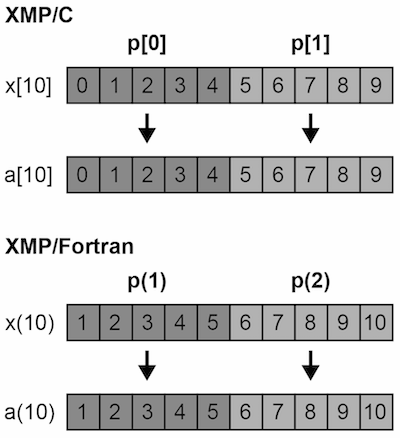
\includegraphics{figs/destributed_array.png}
\end{figure}

But, if you want to use the distributed array in the argument as a
duplicate array in the called procedure, you do not need to redefine
them.

\begin{XCexample}
void sub1(){
#pragma xmp nodes p[2]
#pragma xmp template t[10]
#pragma xmp distribute t[block] onto p
  double x[10];
#pragma xmp align x[i] with t[i]
  sub2(x);
}

void sub2(double a[5]){
  :
}
\end{XCexample}

\begin{XFexample}
subroutine sub1()
!$xmp nodes p(2)
!$xmp template t(10)
!$xmp distribute t(block) onto p
  real x(10)
!$xmp align x(i) with t(i)
  call sub2(x)
end subroutine

subroutine sub2(a)
  real a(5)
  :
end subroutine
\end{XFexample}

\begin{figure}
  \centering
  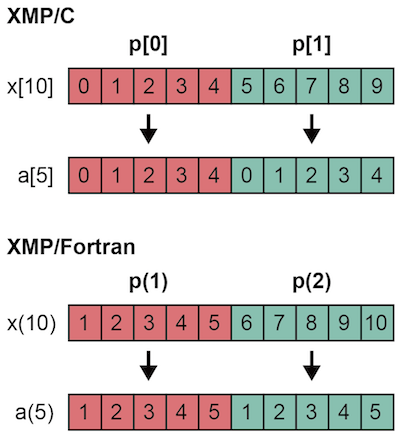
\includegraphics{figs/duplicated_array.png}
\end{figure}